%\chapter{Proof: Existence and uniqueness of solutions}
%\label{Proof:ExistenceUniqueness}




\chapter{Gronwall-inequality}
\label{Gronwall}
Let \(\phi\) and f be nonnegative and continuous functions defined on [0,T]. Let C denote a constant. If:
\[\phi(t)\leq C + \int_0^t \! f(s)\phi(s)\,\mathrm{d}s\quad\text{for all}\:\:t\in[0,T]\]
then:
\[\phi(t)\leq C\cdot\exp(\int_0^t \! f(s)\,\mathrm{d}s) \quad\text{for all}\:\:t\in[0,T].\]
\begin{proof}
See \cite{EvansSDE}.
\end{proof}

\chapter{Code for algorithms and graphics}
\label{code}
We used the programming environment Python 2.7 for the implementation of the algorithms. Especially the packages Matplotlib and Numpy have been very helpful. Informations can be found online. Contact\\
amr.umeri@outlook.com for the source-code.
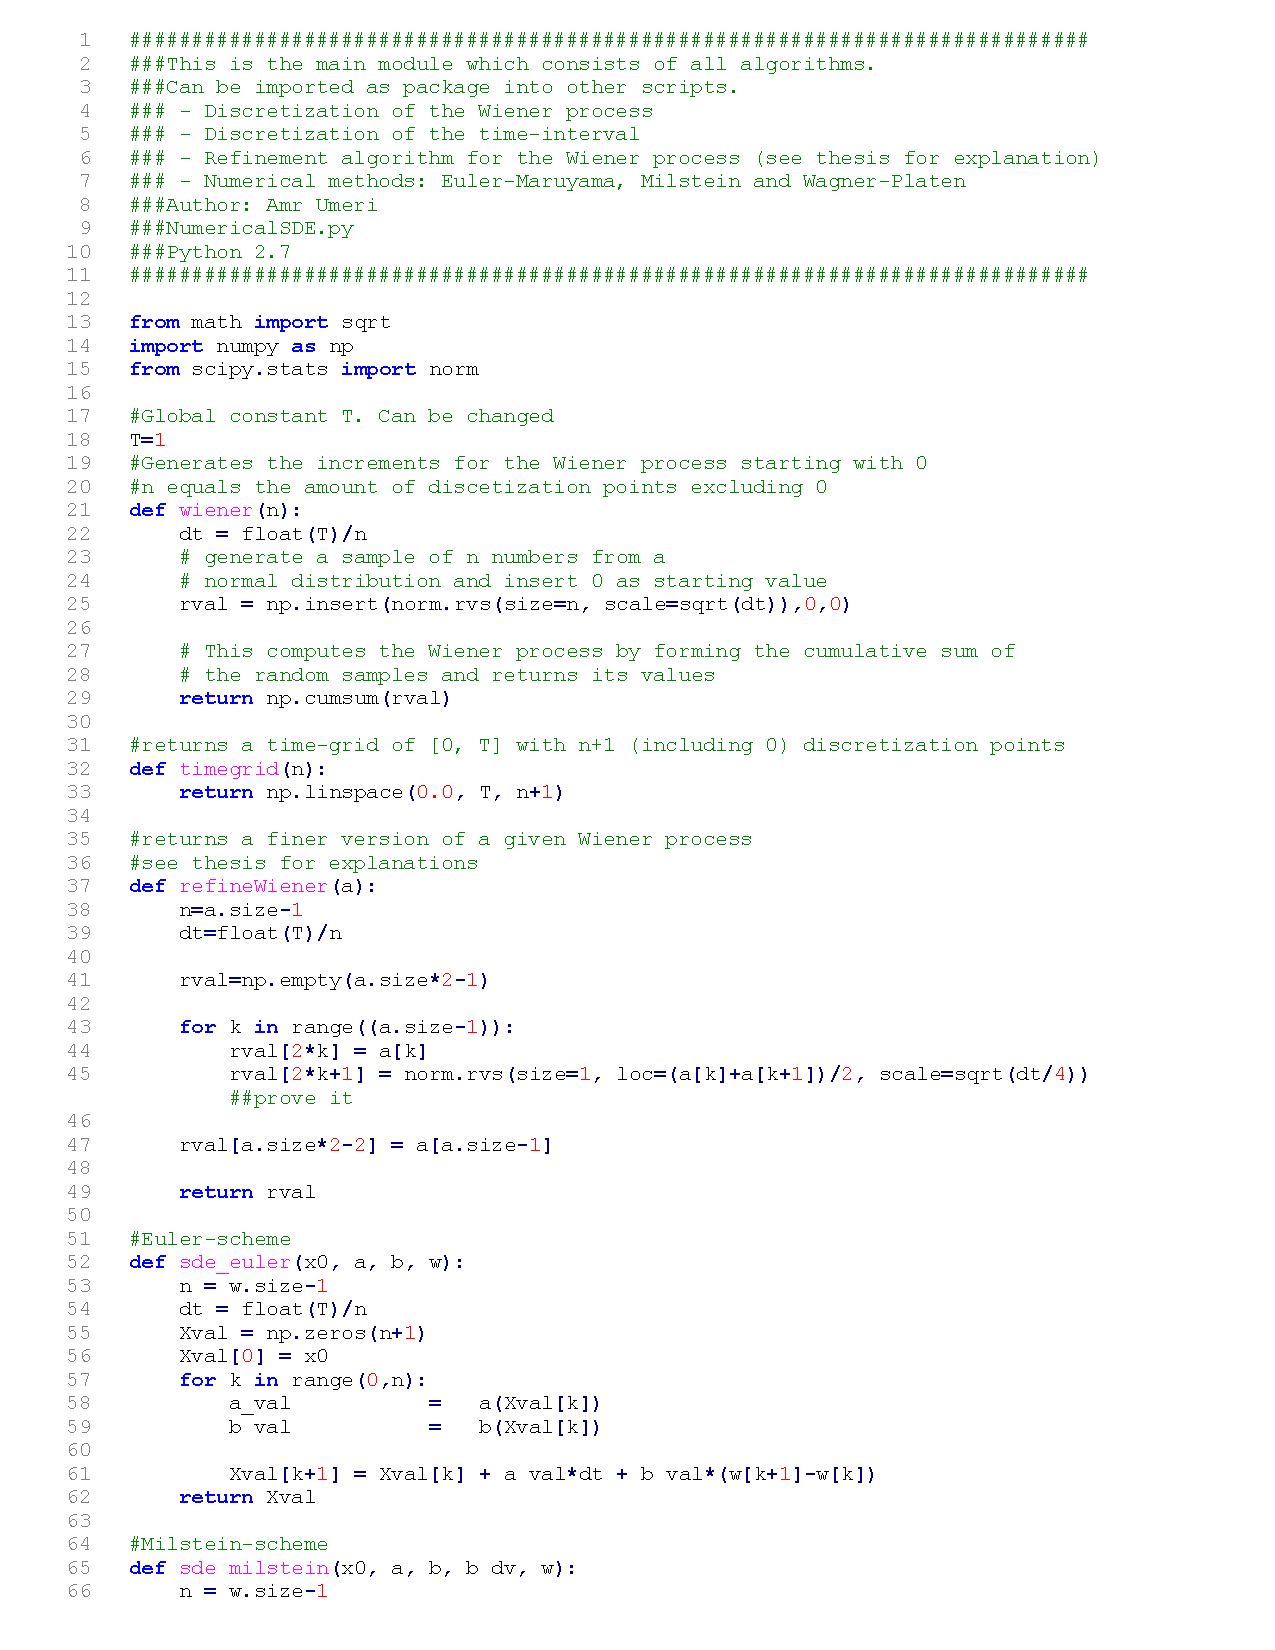
\includepdf[pages={-}]{Content/Code/NumericalSDE.pdf}
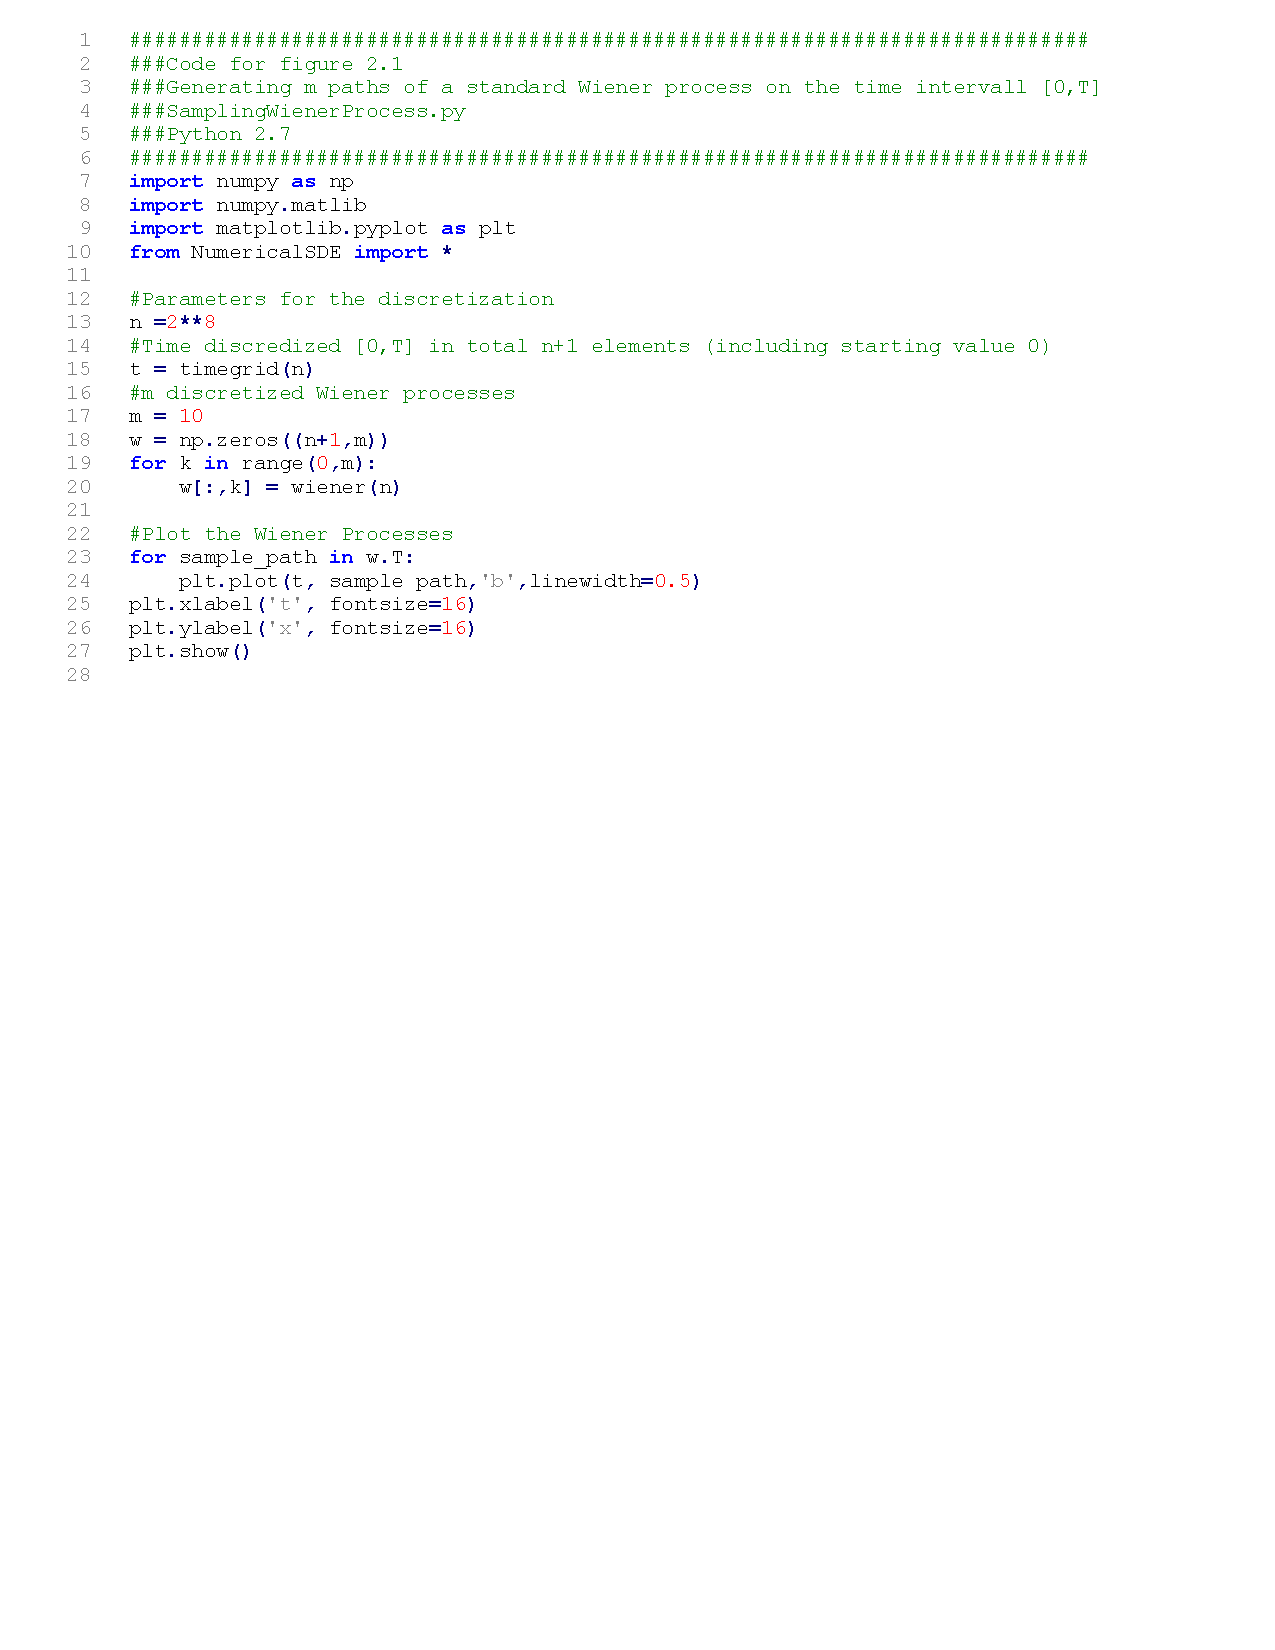
\includepdf[pages={-}]{Content/Code/SamplingWienerProcessGraphic.pdf}
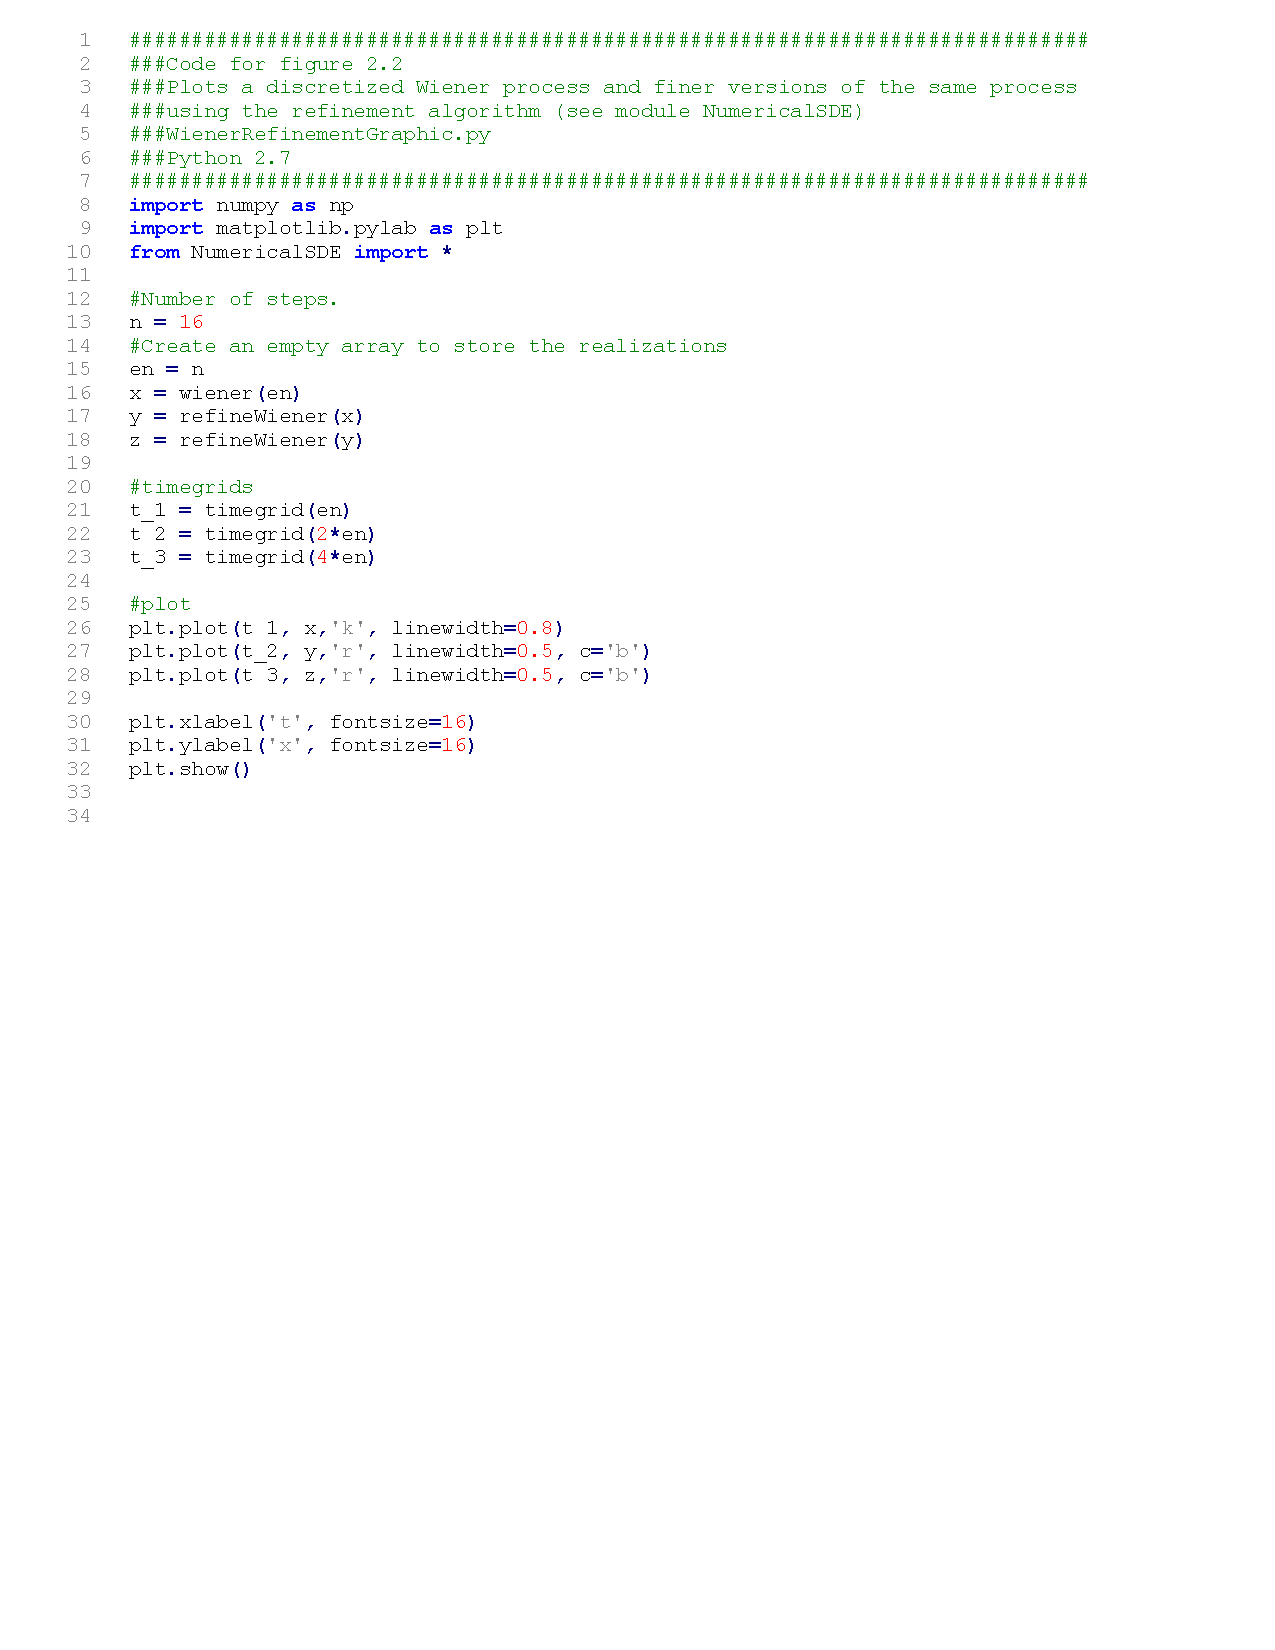
\includepdf[pages={-}]{Content/Code/WienerRefinementGraphic.pdf}
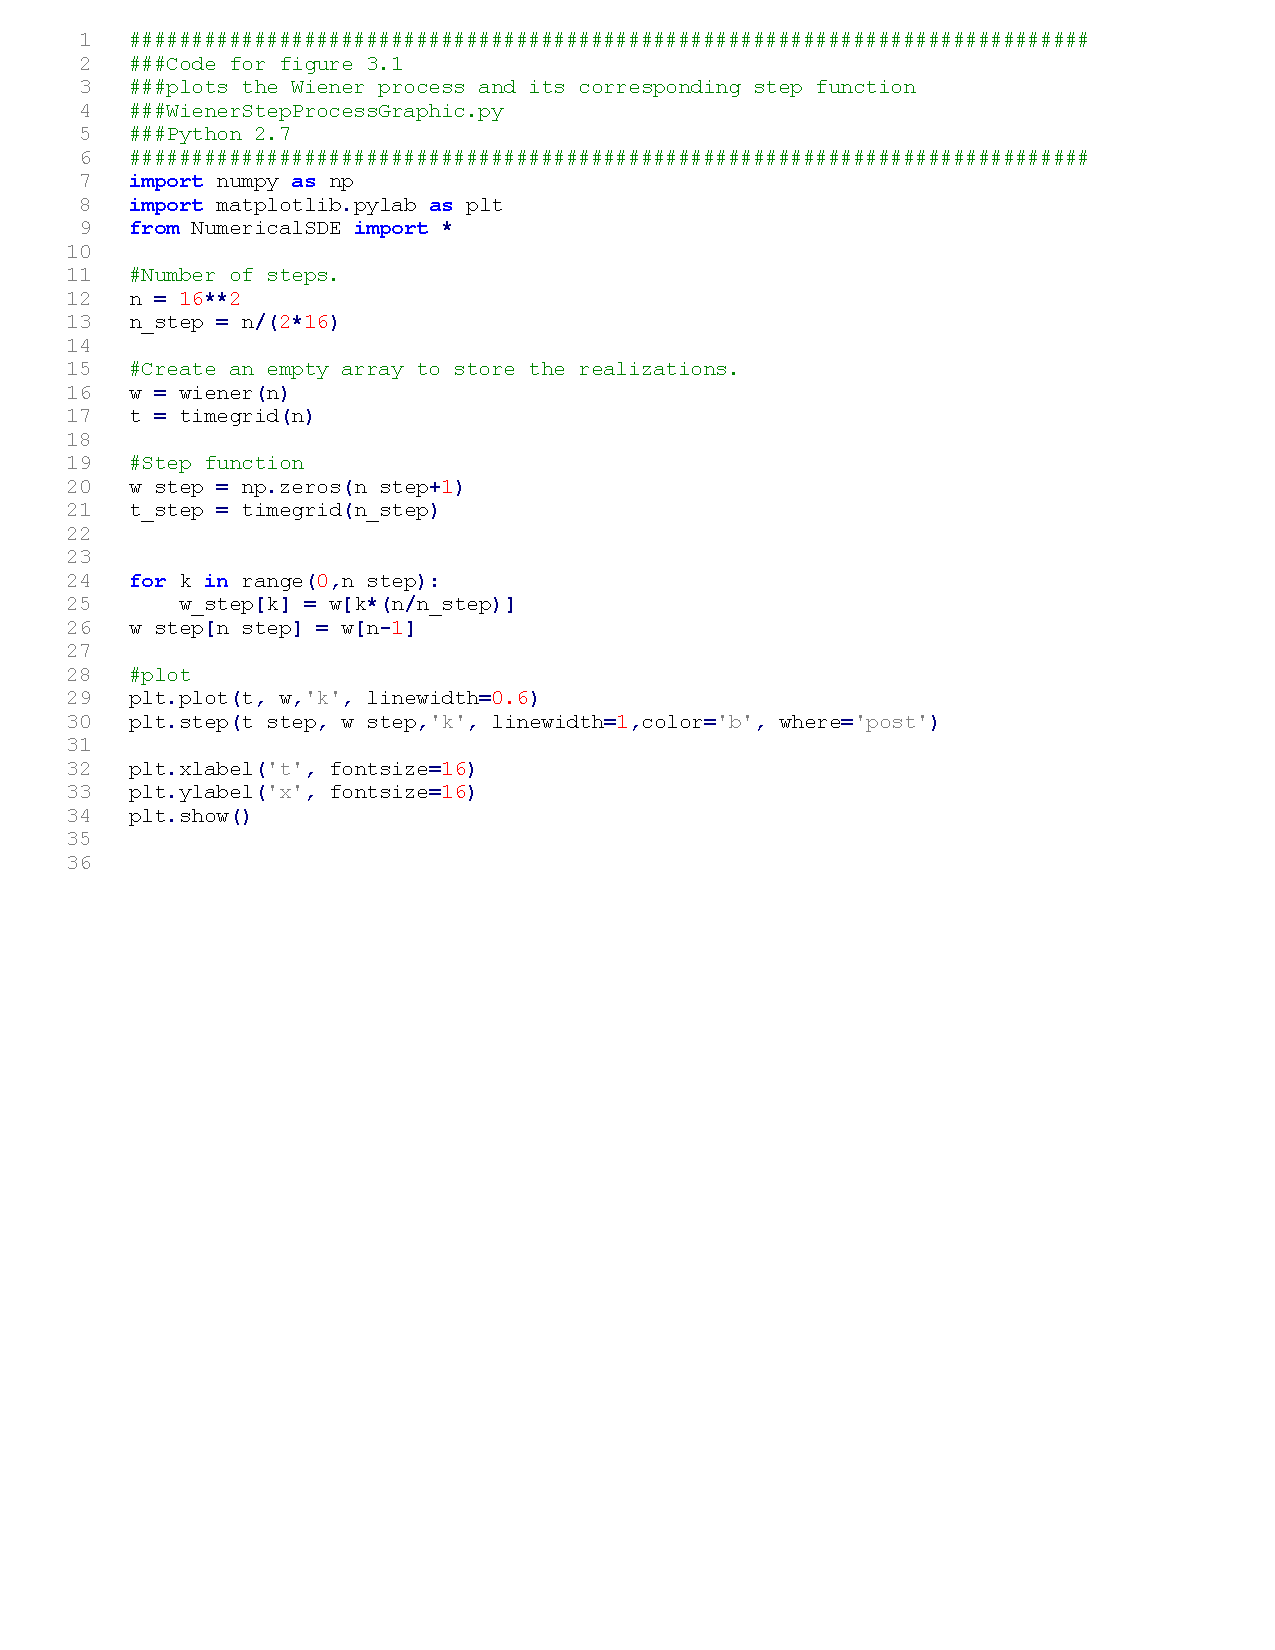
\includepdf[pages={-}]{Content/Code/WienerStepProcessGraphic.pdf}
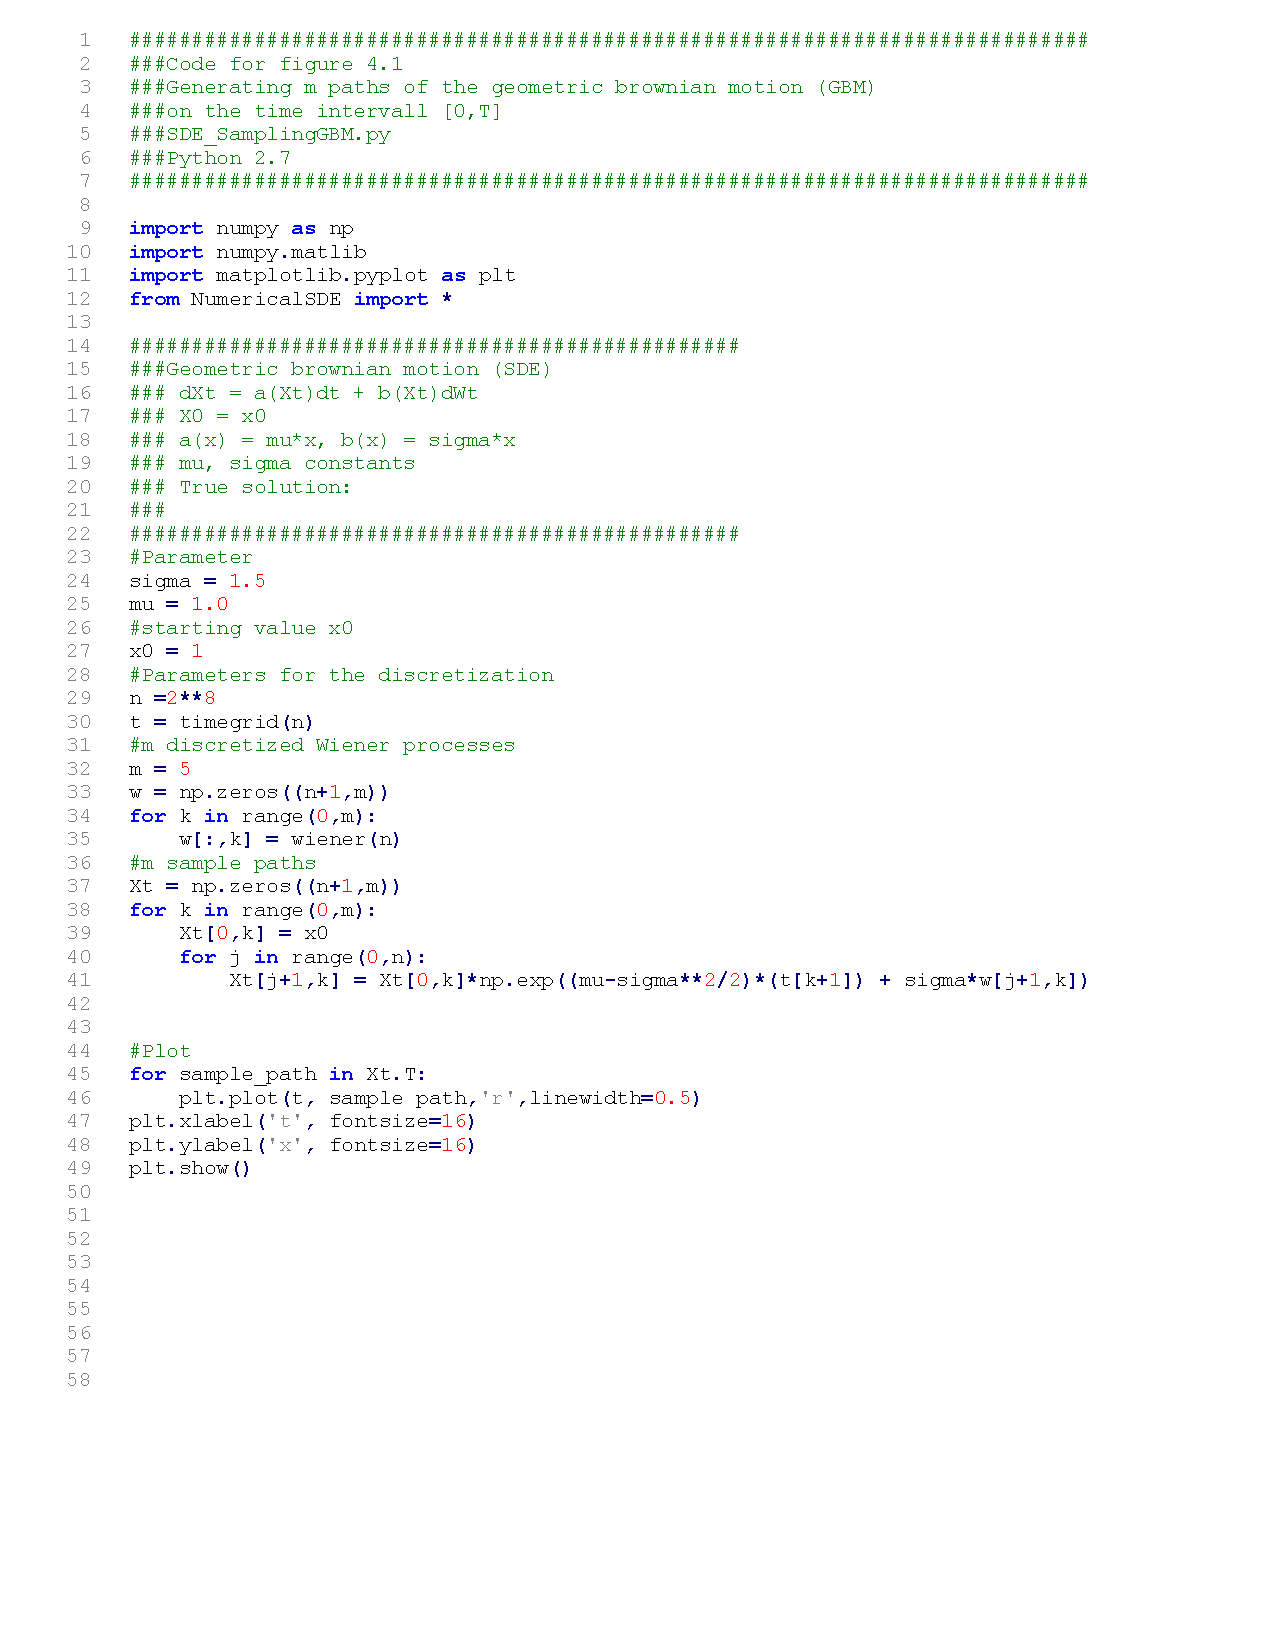
\includepdf[pages={-}]{Content/Code/SDE_SamplingGBM.pdf}
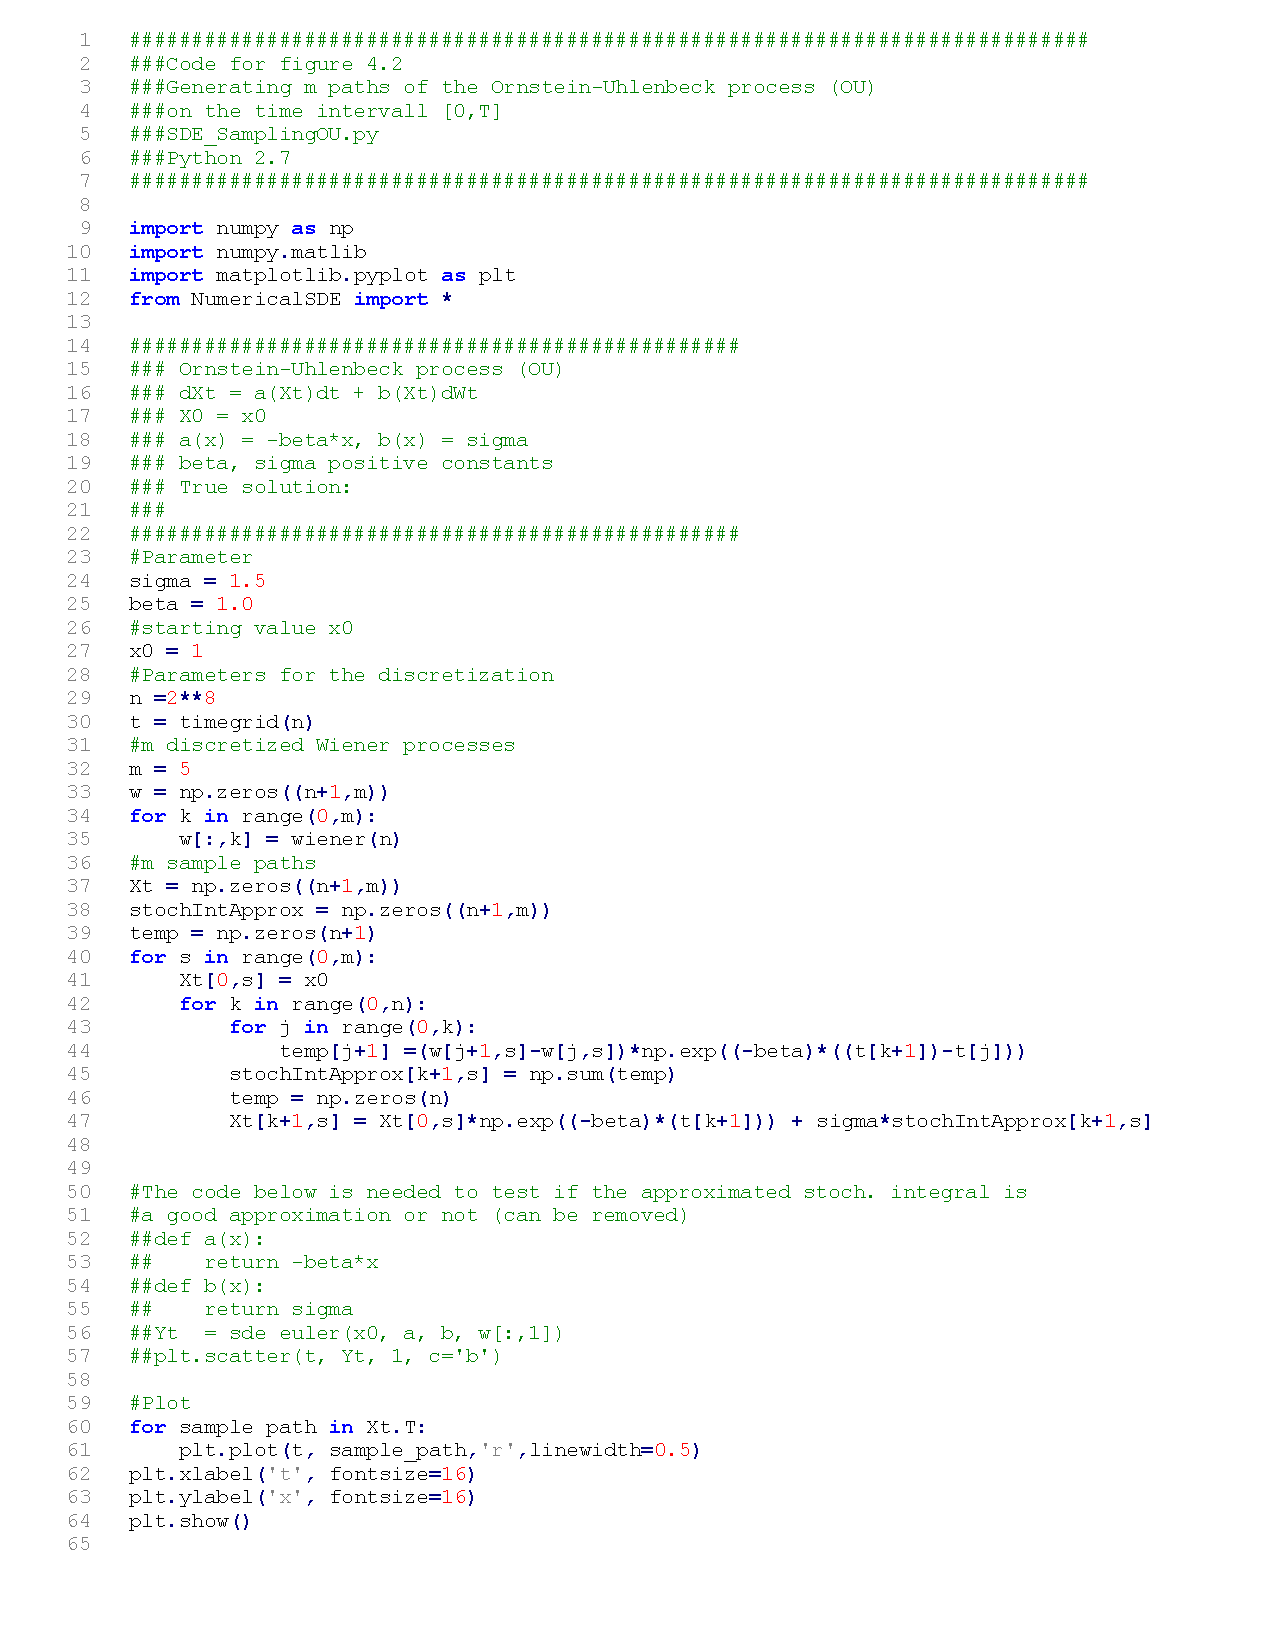
\includepdf[pages={-}]{Content/Code/SDE_SamplingOU.pdf}
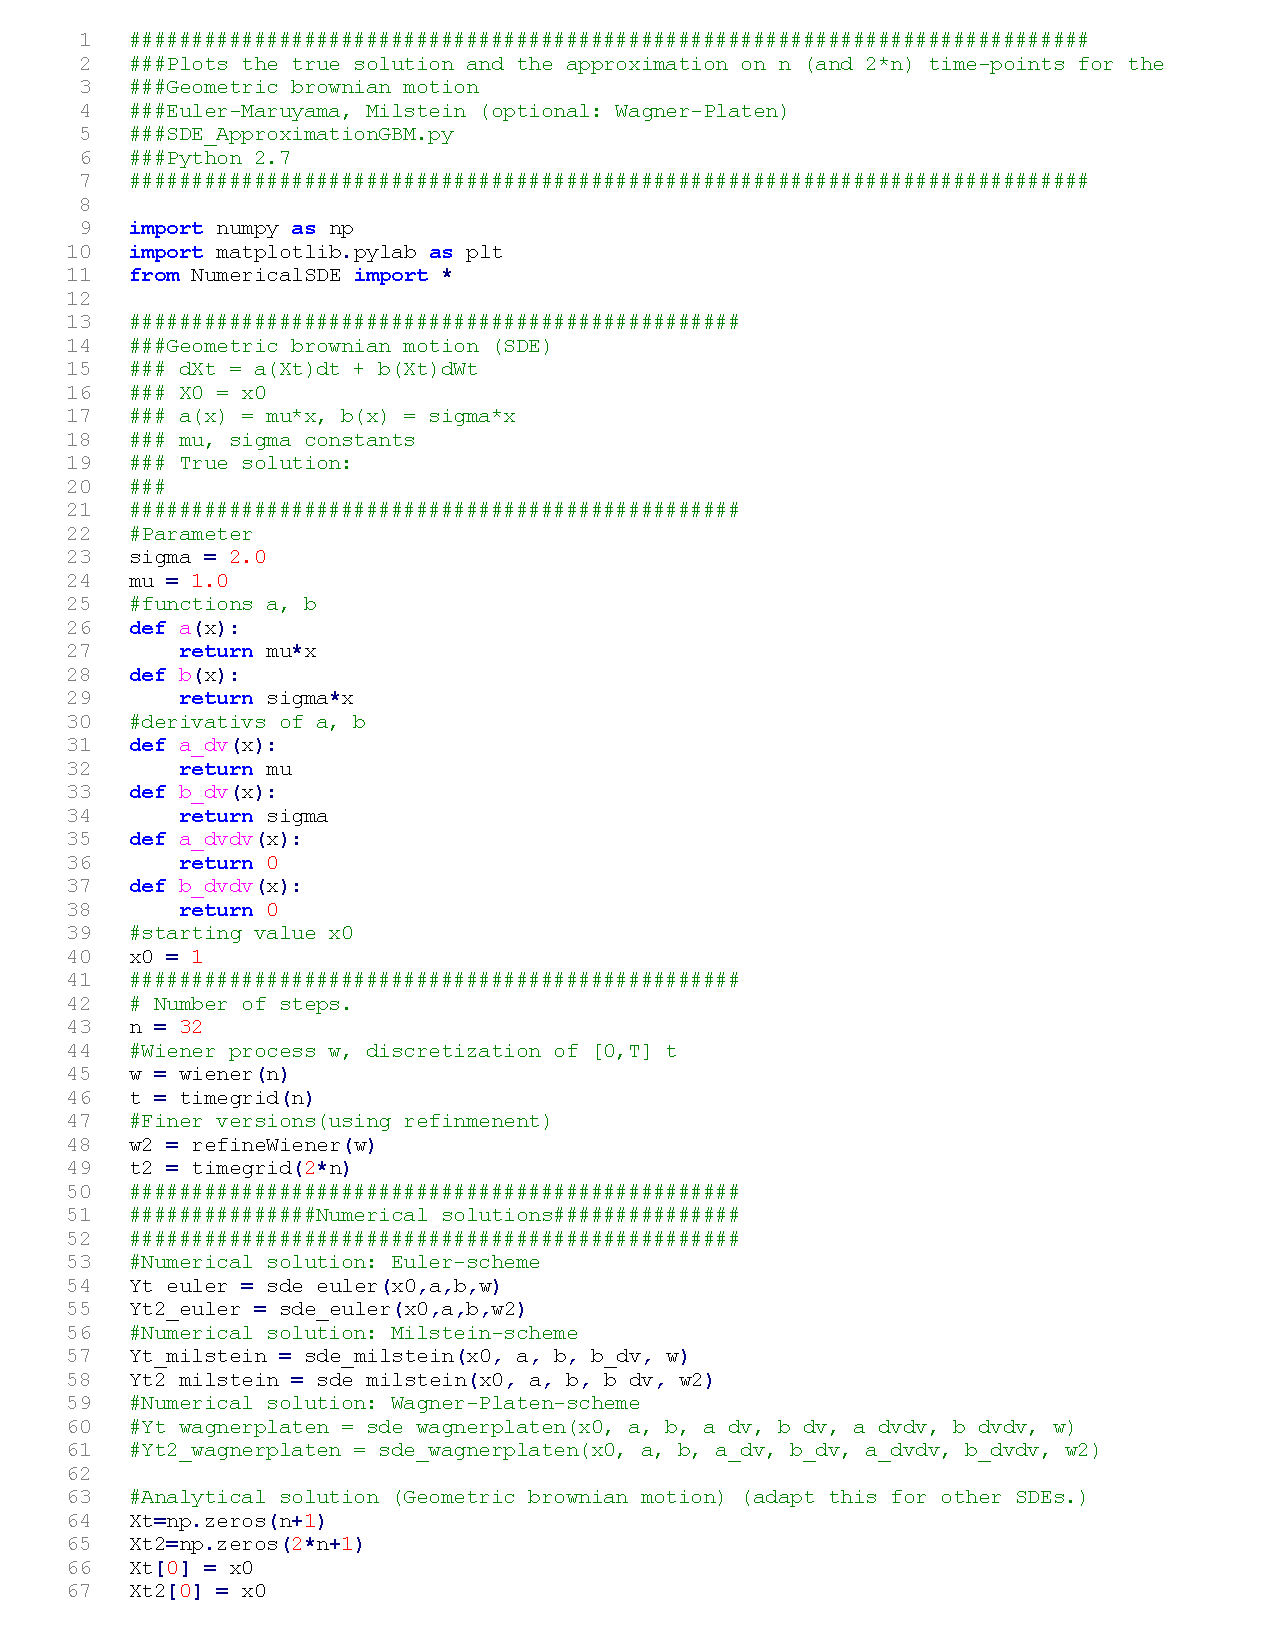
\includepdf[pages={-}]{Content/Code/SDE_ApproximationGBM.pdf}
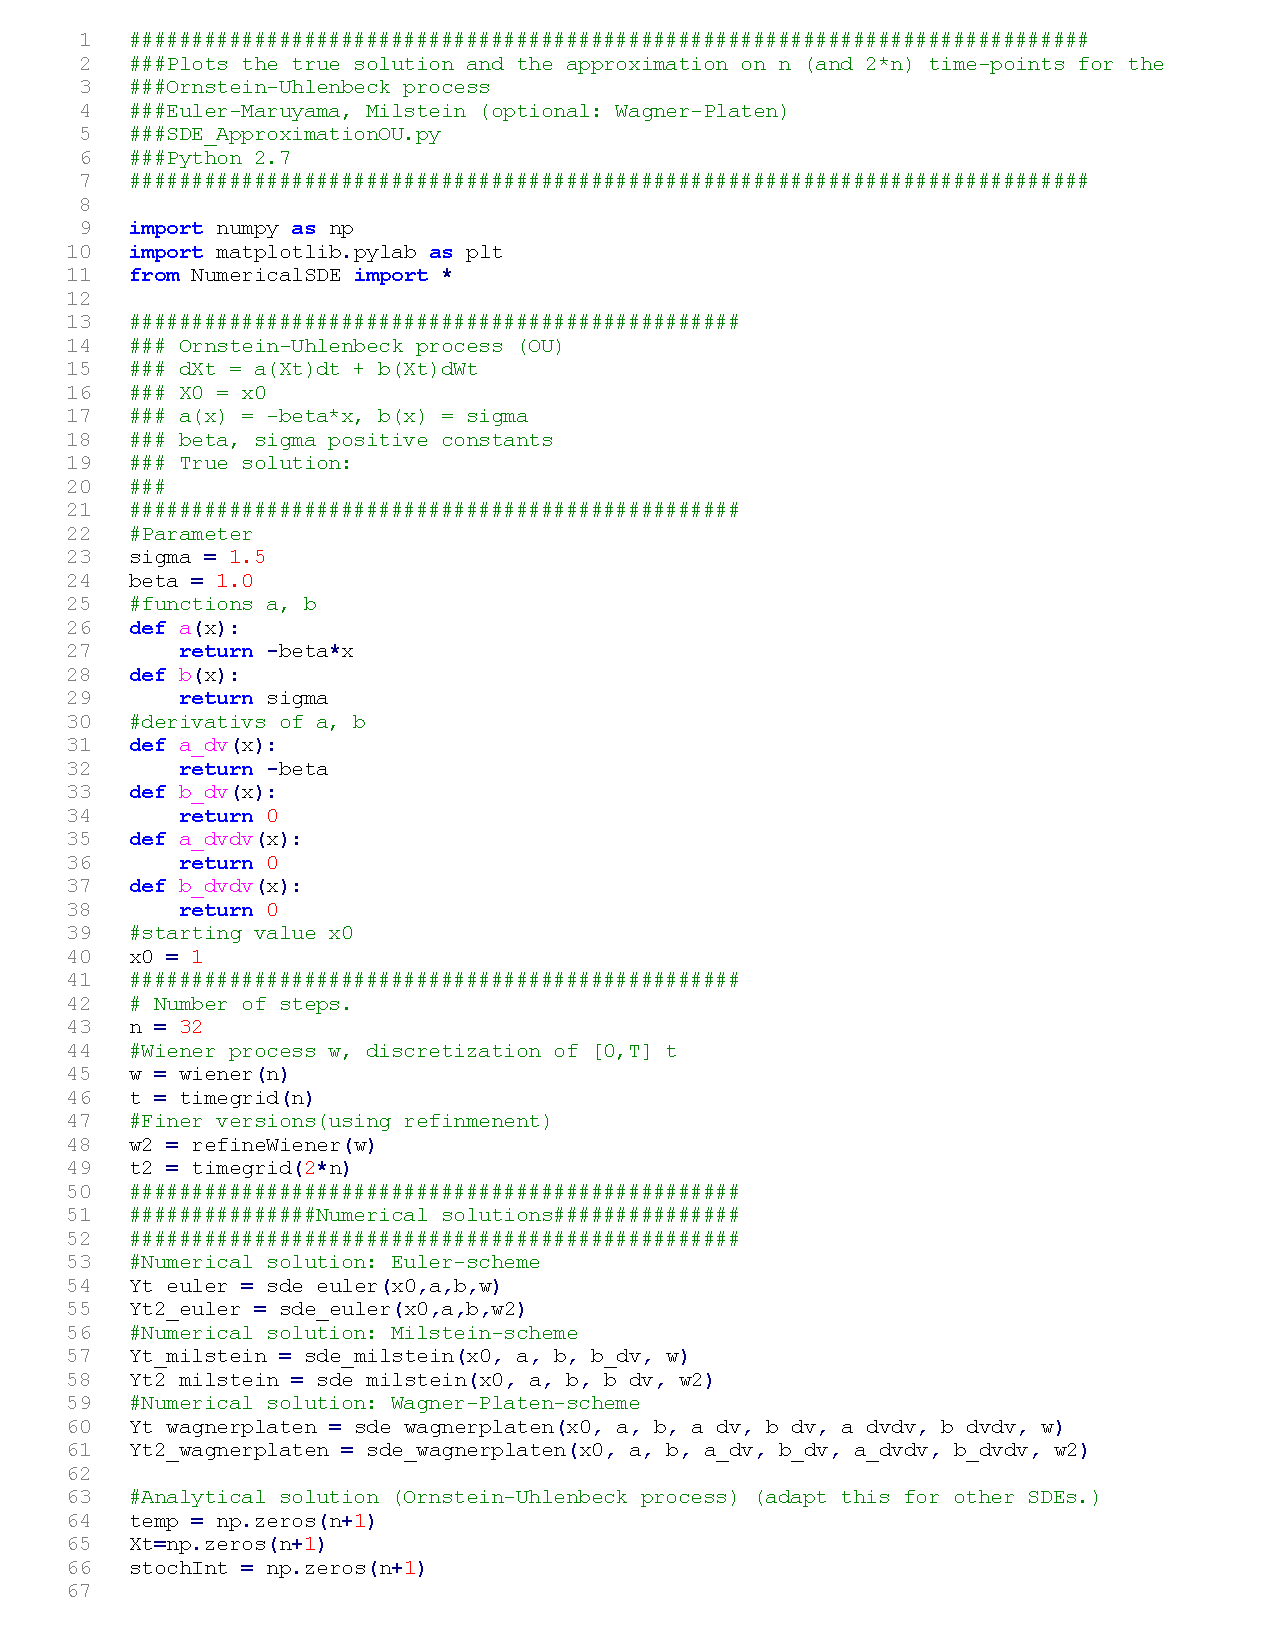
\includepdf[pages={-}]{Content/Code/SDE_ApproximationOU.pdf}
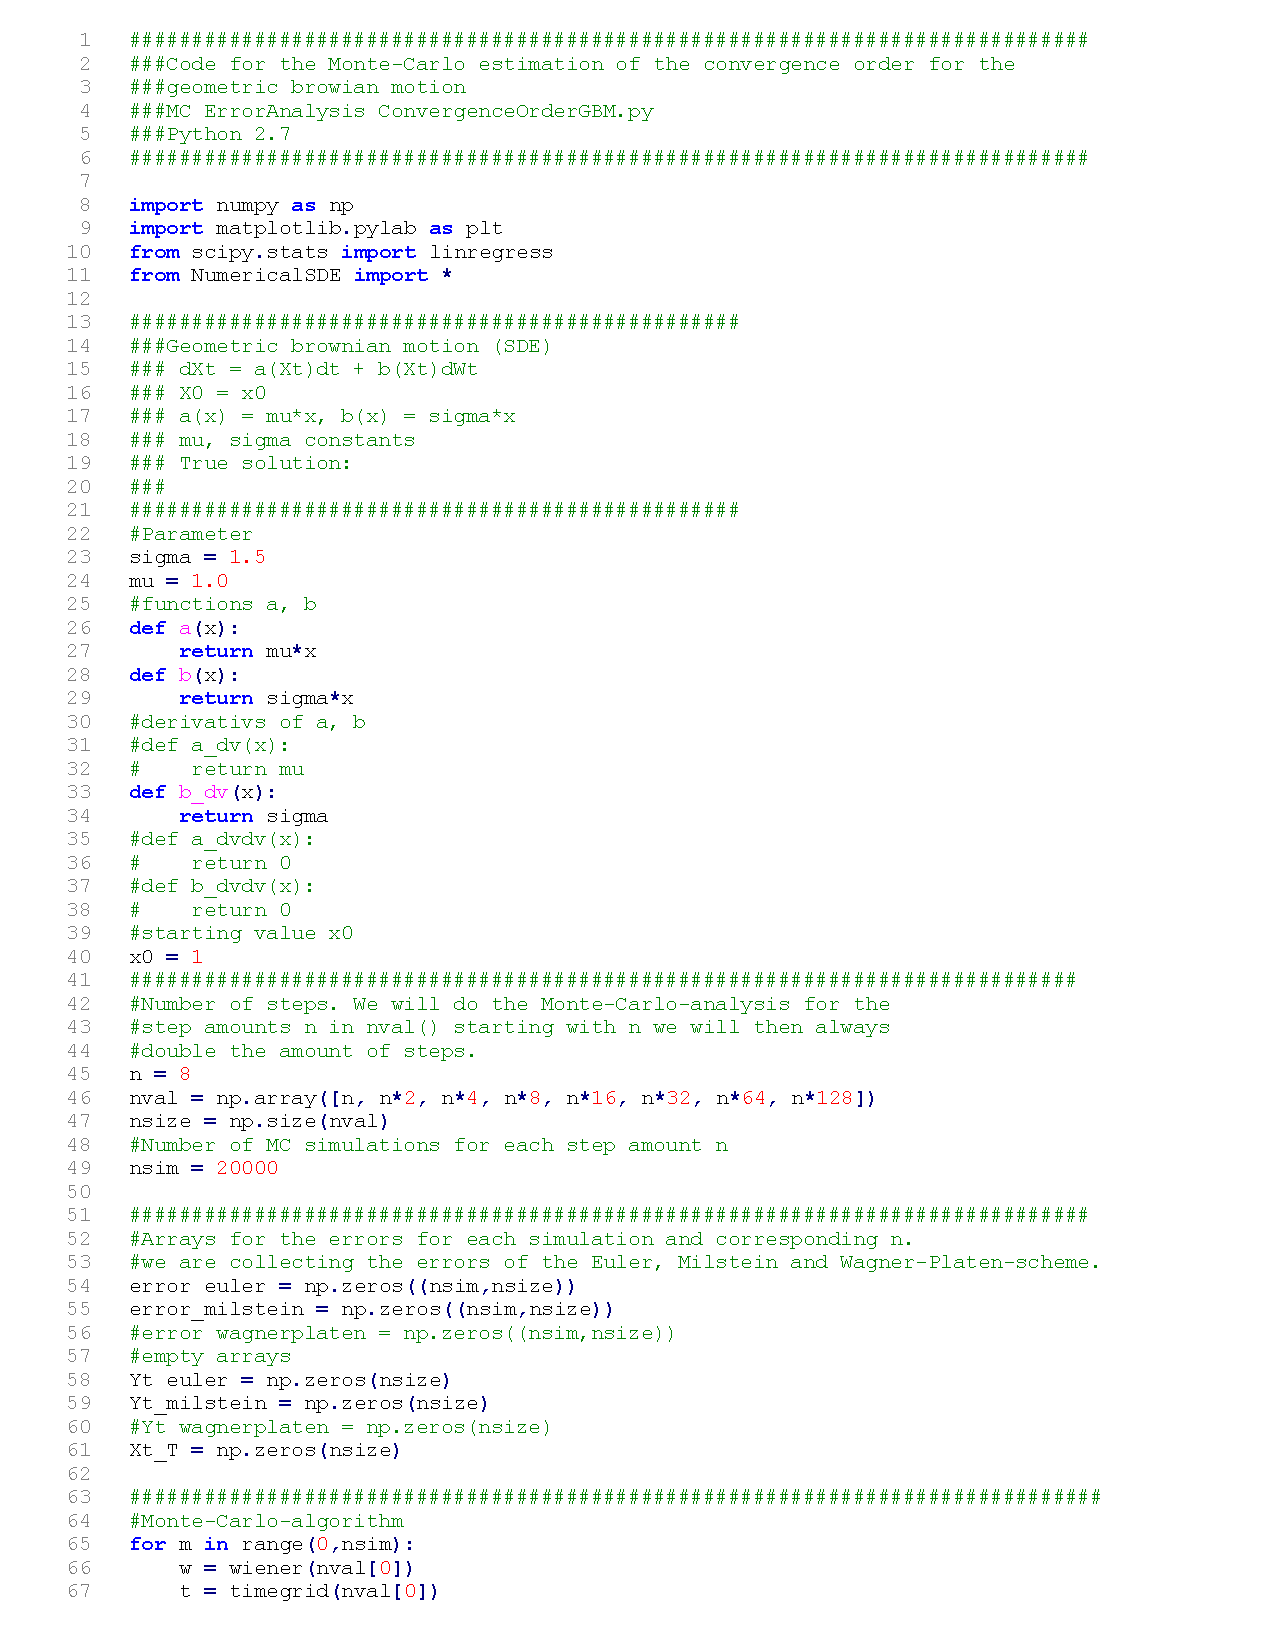
\includepdf[pages={-}]{Content/Code/MC_ConvergenceOrderGBM.pdf}
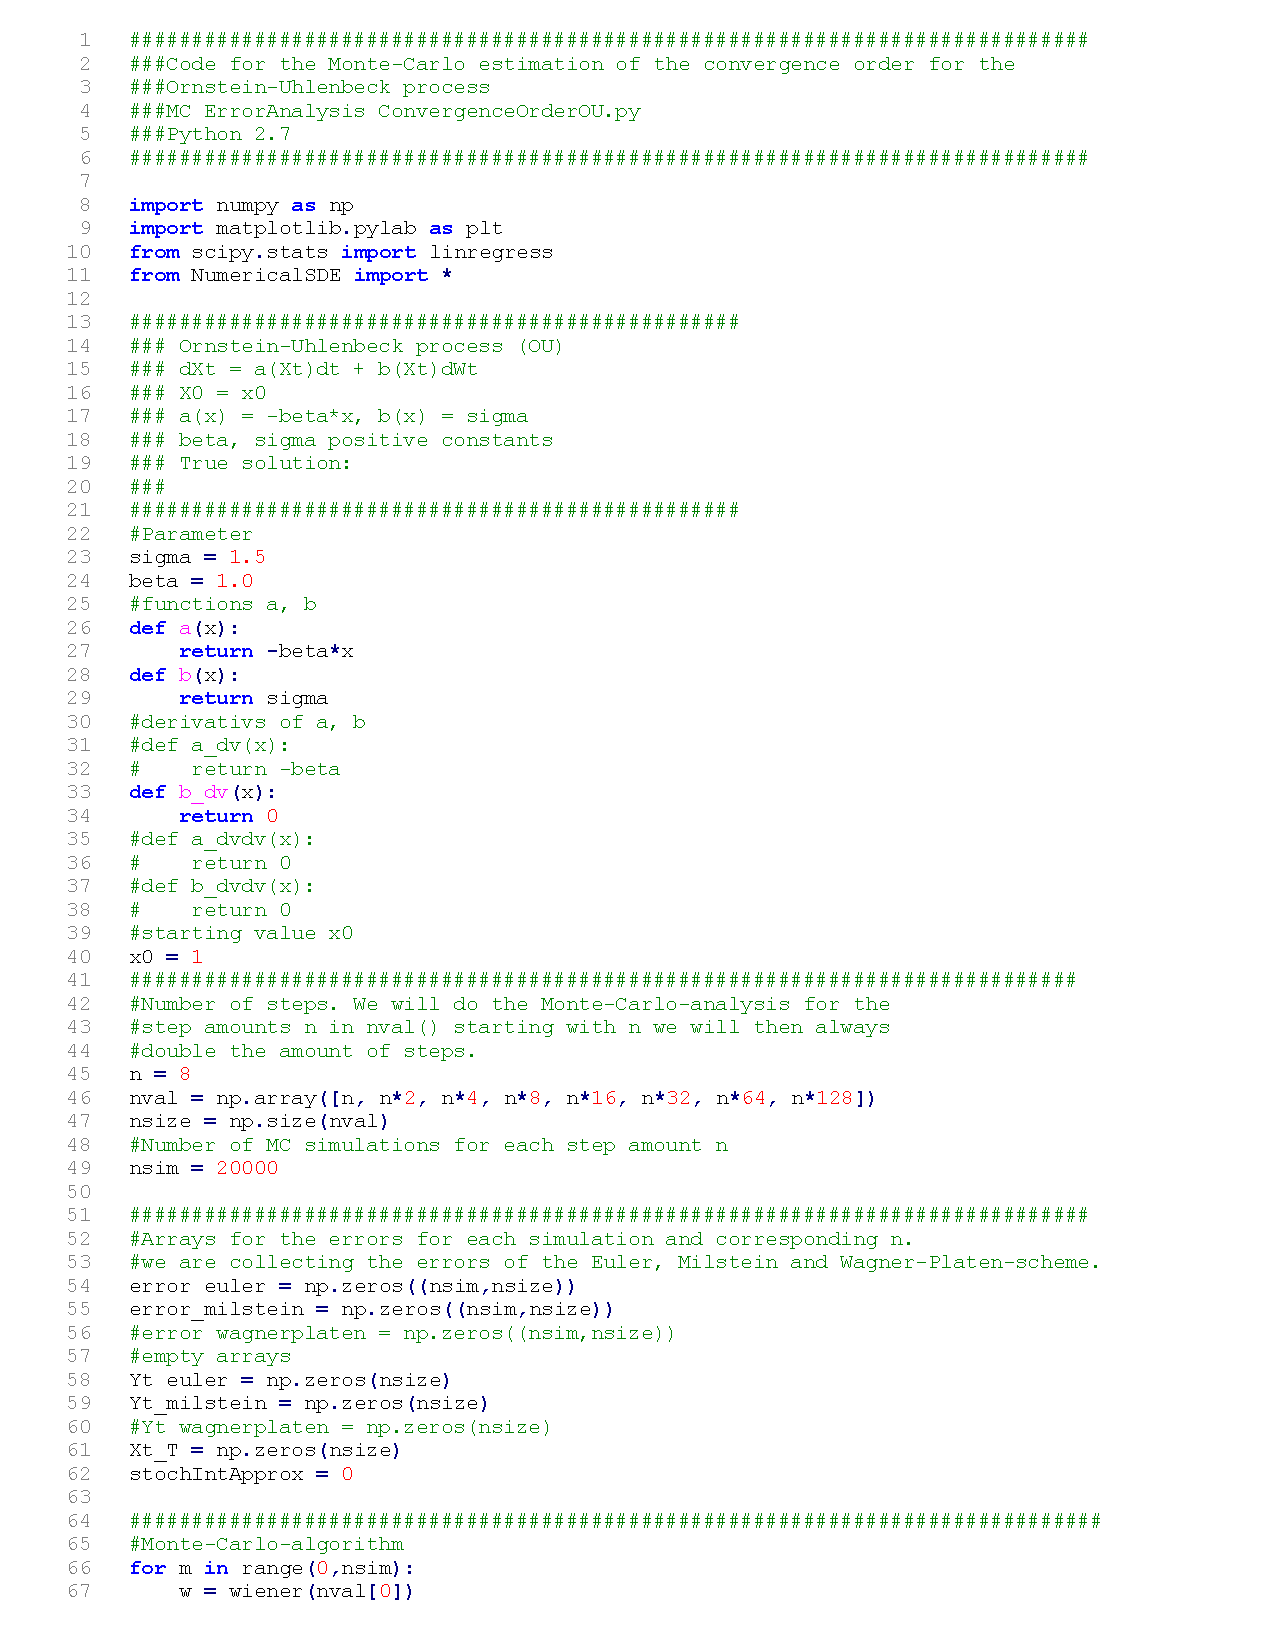
\includepdf[pages={-}]{Content/Code/MC_ConvergenceOrderOU.pdf}


\chapter{Additional graphics}
\label{Graphics}
We included some additional figures in the next pages to illustrate the approximation schemes. Especially we also added some graphics of the Wagner-Platen approximation and its error-analysis. It has strong order 1.5. This scheme has not beed discussed in the main text of the thesis. However we implemented this scheme as well.


\begin{figure}[!h]
\centering
   \begin{subfigure}{0.49\linewidth} \centering
     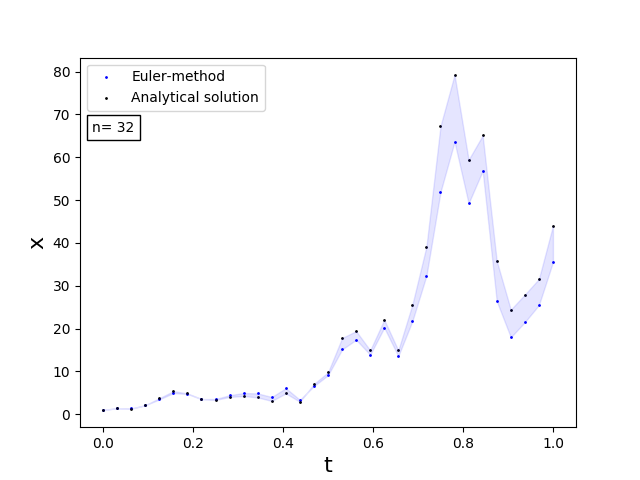
\includegraphics[scale=0.4]{Content/Graphics/Appendix/1gbm}
   \end{subfigure}
   \begin{subfigure}{0.49\linewidth} \centering
     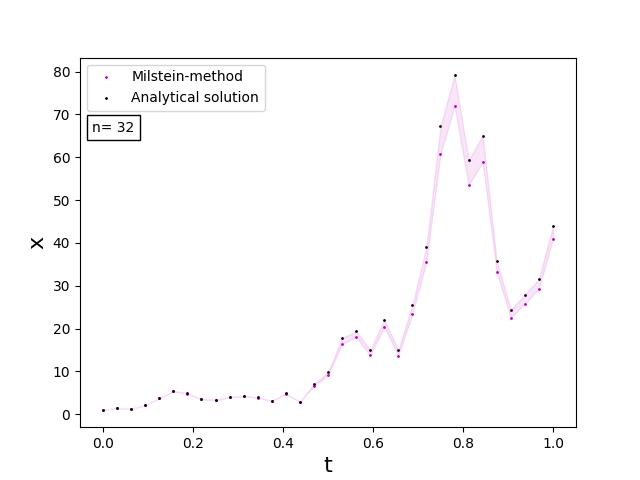
\includegraphics[scale=0.4]{Content/Graphics/Appendix/2gbm}
   \end{subfigure}
   \begin{subfigure}{0.49\linewidth} \centering
     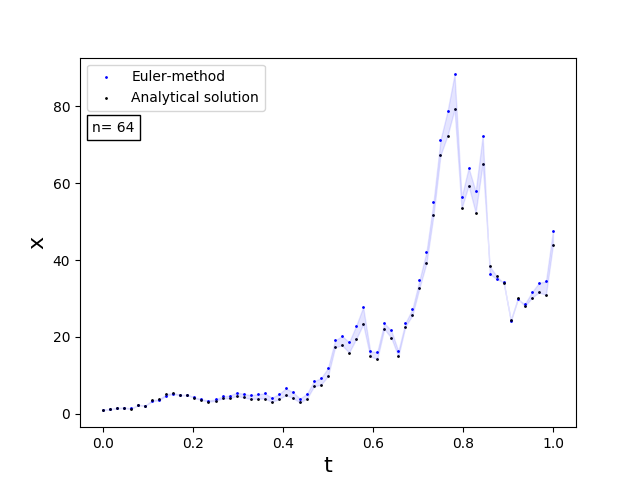
\includegraphics[scale=0.4]{Content/Graphics/Appendix/3gbm}
   \end{subfigure}
   \begin{subfigure}{0.49\linewidth} \centering
     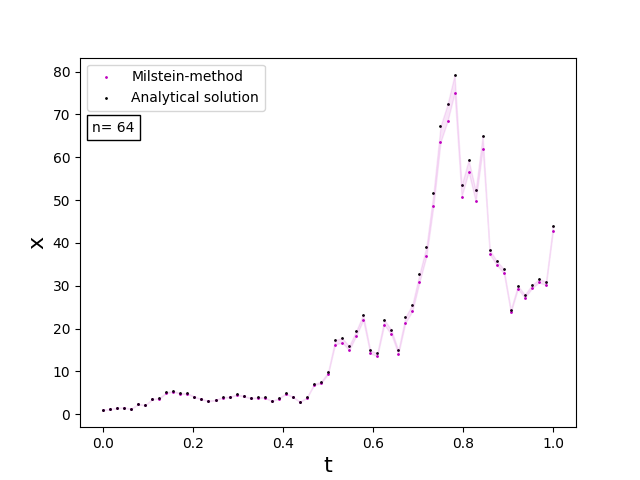
\includegraphics[scale=0.4]{Content/Graphics/Appendix/4gbm}
   \end{subfigure}
   \begin{subfigure}{0.49\linewidth} \centering
     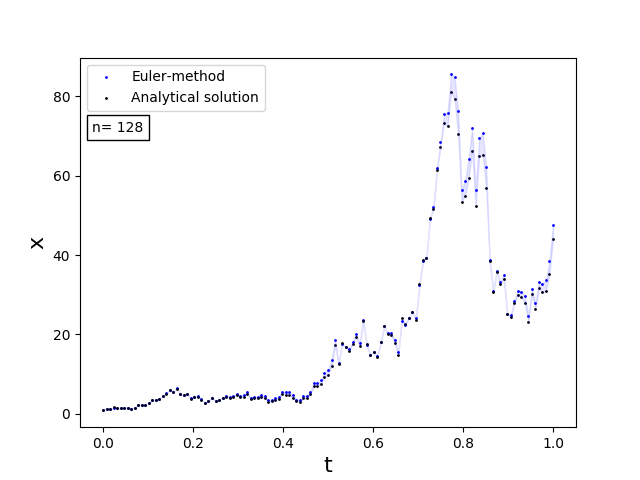
\includegraphics[scale=0.4]{Content/Graphics/Appendix/5gbm}
   \end{subfigure}
   \begin{subfigure}{0.49\linewidth} \centering
     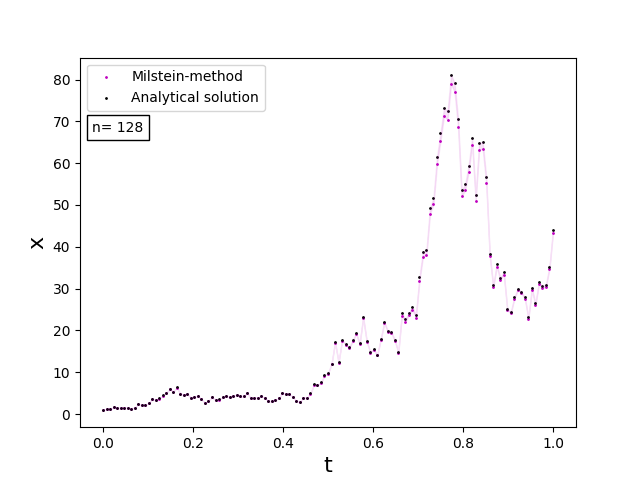
\includegraphics[scale=0.4]{Content/Graphics/Appendix/6gbm}
   \end{subfigure}
\caption{Approximation (colored dots) of the sample path of the geometric Brownian motion and the true sample path (black dots) for n = 32, 64, 128 using Euler and Milstein.}
\end{figure}

\begin{figure}[!h]
\centering
   \begin{subfigure}{0.49\linewidth} \centering
     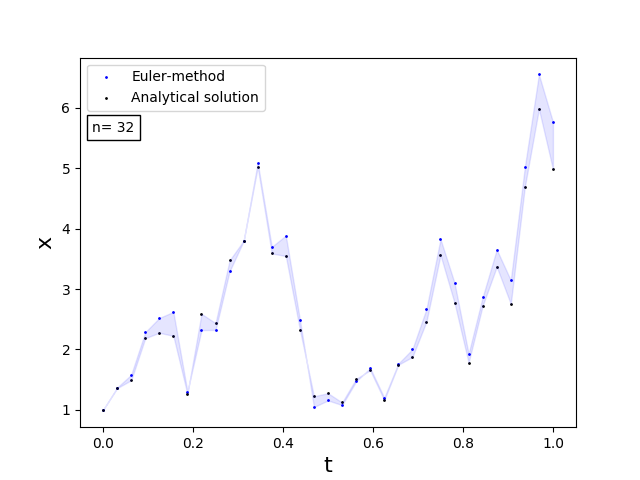
\includegraphics[scale=0.4]{Content/Graphics/Appendix/1gbm2}
   \end{subfigure}
   \begin{subfigure}{0.49\linewidth} \centering
     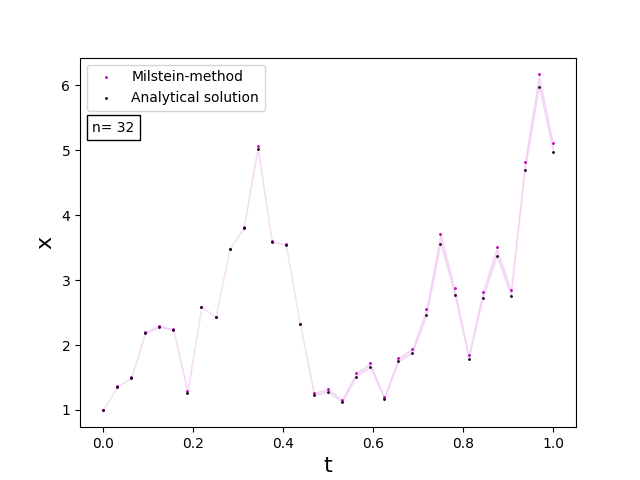
\includegraphics[scale=0.4]{Content/Graphics/Appendix/2gbm2}
   \end{subfigure}
   \begin{subfigure}{0.49\linewidth} \centering
     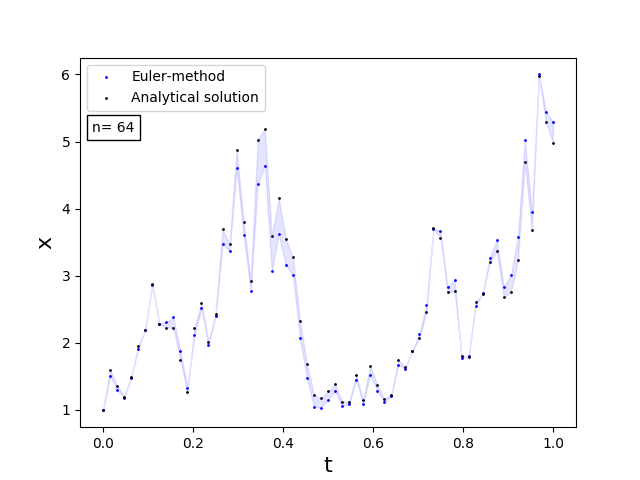
\includegraphics[scale=0.4]{Content/Graphics/Appendix/3gbm2}
   \end{subfigure}
   \begin{subfigure}{0.49\linewidth} \centering
     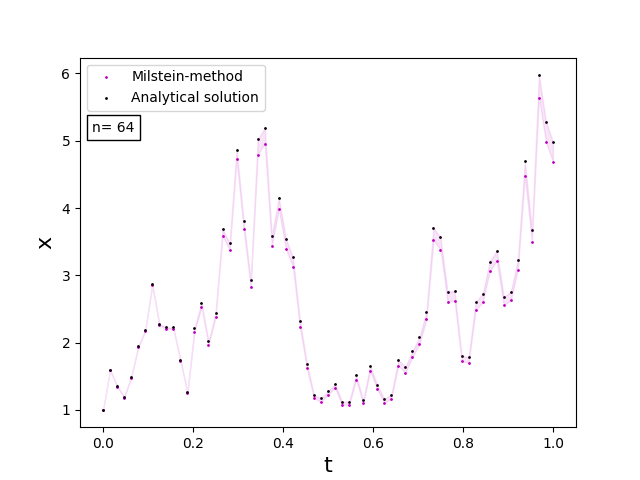
\includegraphics[scale=0.4]{Content/Graphics/Appendix/4gbm2}
   \end{subfigure}
   \begin{subfigure}{0.49\linewidth} \centering
     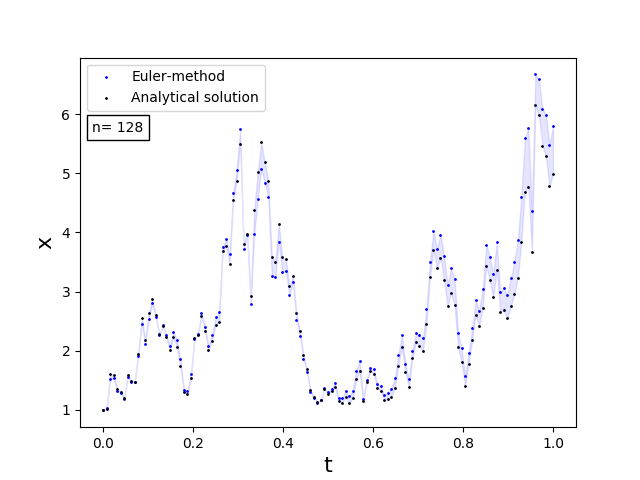
\includegraphics[scale=0.4]{Content/Graphics/Appendix/5gbm2}
   \end{subfigure}
   \begin{subfigure}{0.49\linewidth} \centering
     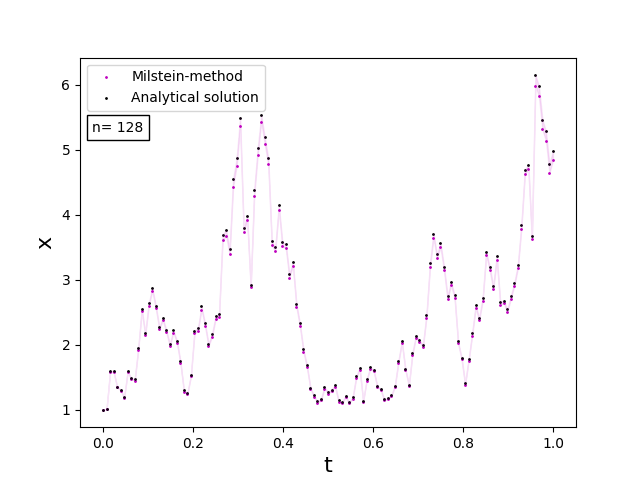
\includegraphics[scale=0.4]{Content/Graphics/Appendix/6gbm2}
   \end{subfigure}
\caption{Approximation (colored dots) of the sample path of the geometric Brownian motion and the true sample path (black dots) for n = 32, 64, 128 using Euler and Milstein.}
\end{figure}


\begin{figure}[!h]
\centering
   \begin{subfigure}{0.49\linewidth} \centering
     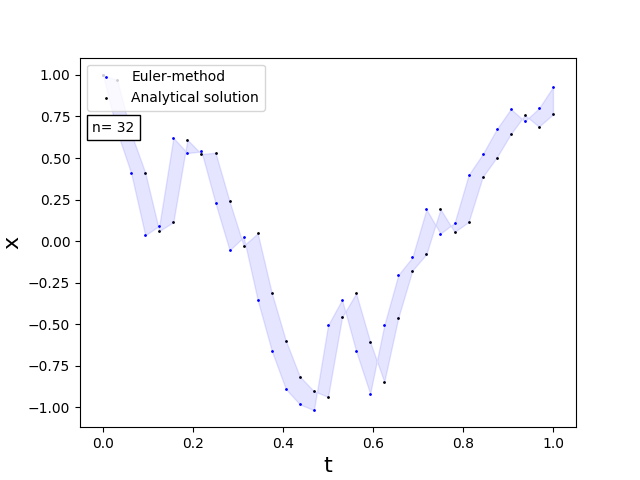
\includegraphics[scale=0.4]{Content/Graphics/Appendix/1ou}
   \end{subfigure}
   \begin{subfigure}{0.49\linewidth} \centering
     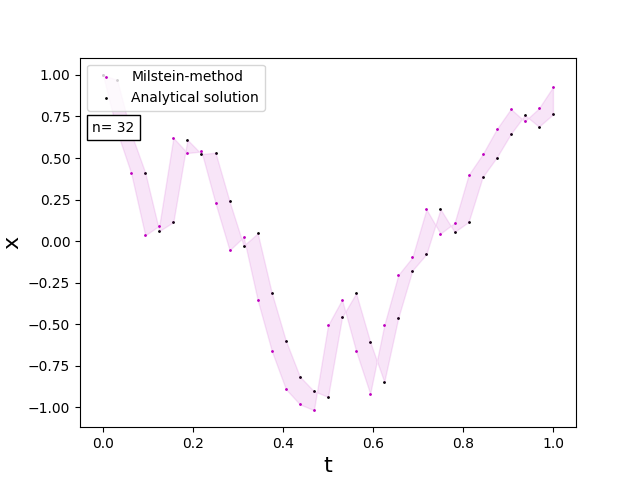
\includegraphics[scale=0.4]{Content/Graphics/Appendix/2ou}
   \end{subfigure}
   \begin{subfigure}{0.49\linewidth} \centering
     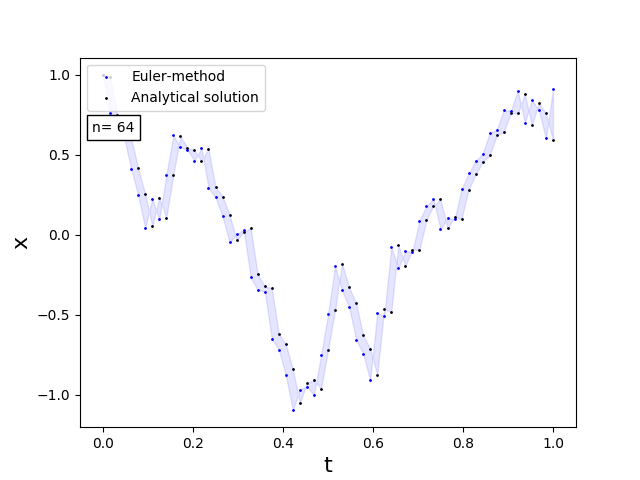
\includegraphics[scale=0.4]{Content/Graphics/Appendix/3ou}
   \end{subfigure}
   \begin{subfigure}{0.49\linewidth} \centering
     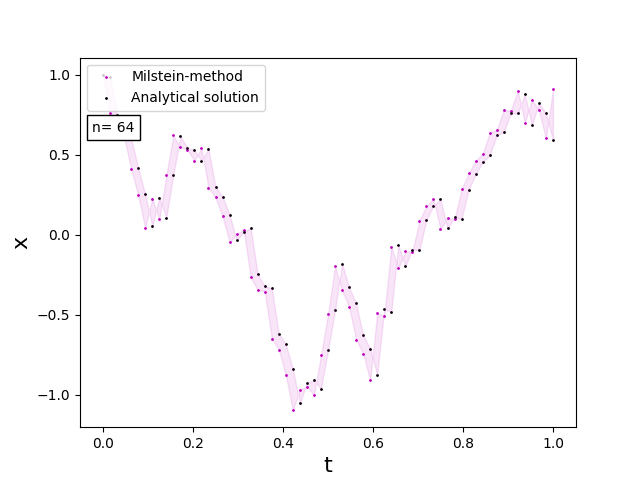
\includegraphics[scale=0.4]{Content/Graphics/Appendix/4ou}
   \end{subfigure}
   \begin{subfigure}{0.49\linewidth} \centering
     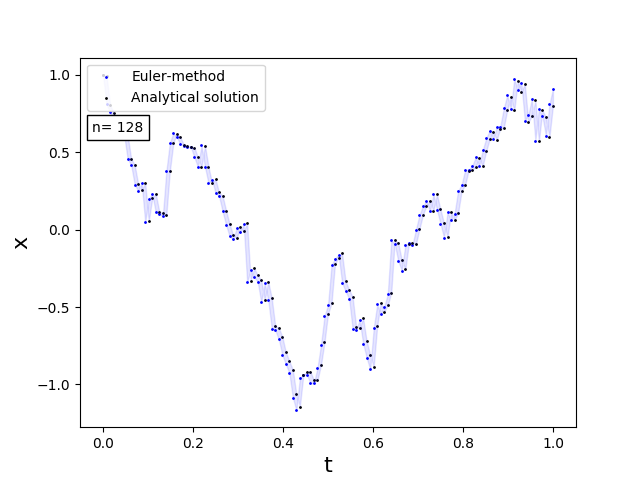
\includegraphics[scale=0.4]{Content/Graphics/Appendix/5ou}
   \end{subfigure}
   \begin{subfigure}{0.49\linewidth} \centering
     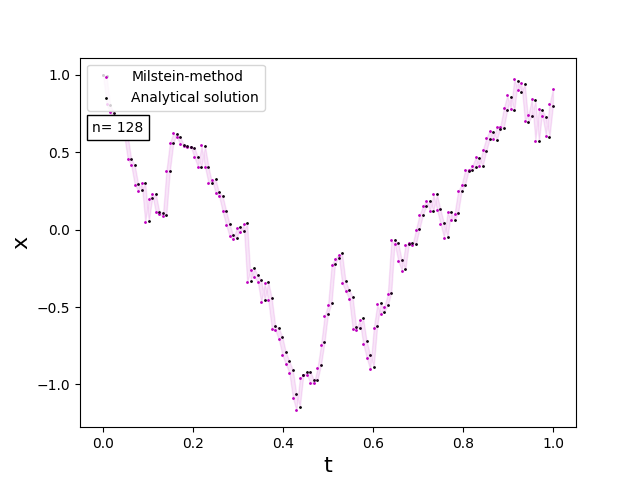
\includegraphics[scale=0.4]{Content/Graphics/Appendix/6ou}
   \end{subfigure}
\caption{Approximation (colored dots) of the sample path of the Ornstein-Uhlenbeck process and the true sample path (black dots) for n = 32, 64, 128 using Euler and Milstein.}
\end{figure}


\begin{figure}[!h]
\centering
   \begin{subfigure}{0.49\linewidth} \centering
     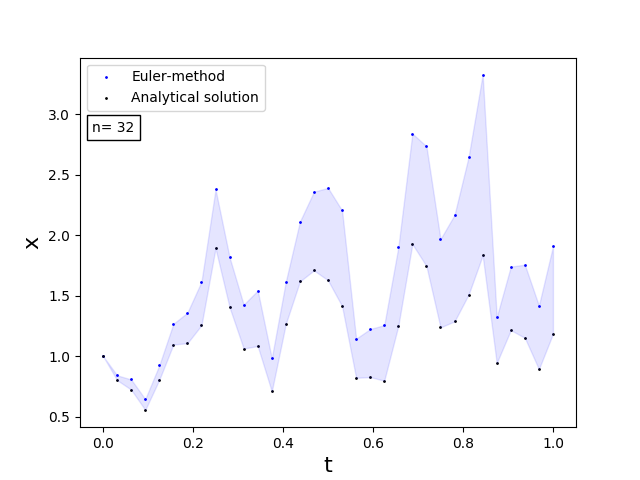
\includegraphics[scale=0.4]{Content/Graphics/Appendix/1gbm3}
   \end{subfigure}
   \begin{subfigure}{0.49\linewidth} \centering
     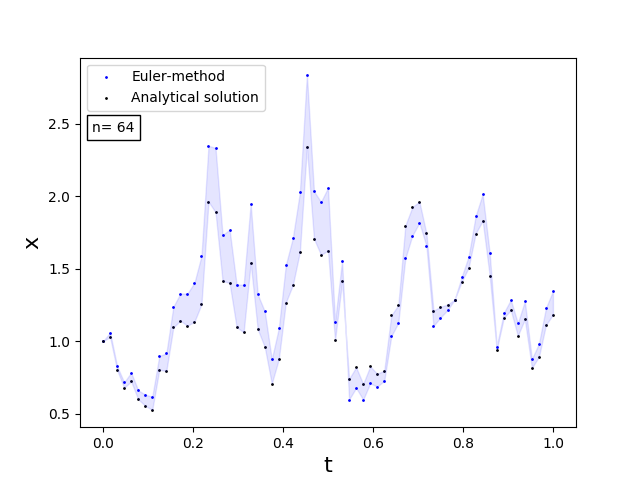
\includegraphics[scale=0.4]{Content/Graphics/Appendix/4gbm3}
   \end{subfigure}
   \begin{subfigure}{0.49\linewidth} \centering
     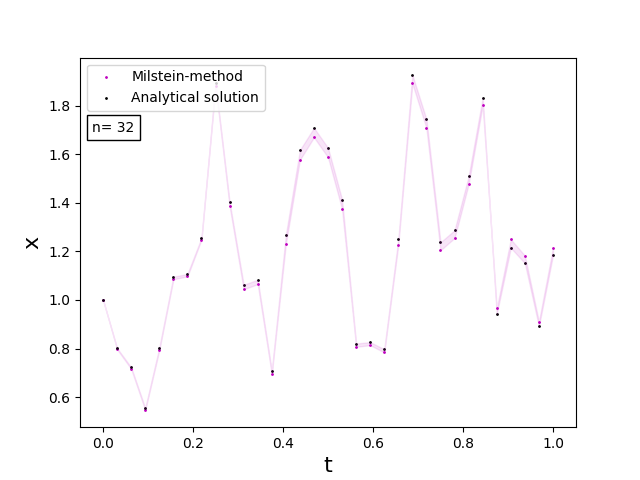
\includegraphics[scale=0.4]{Content/Graphics/Appendix/2gbm3}
   \end{subfigure}
   \begin{subfigure}{0.49\linewidth} \centering
     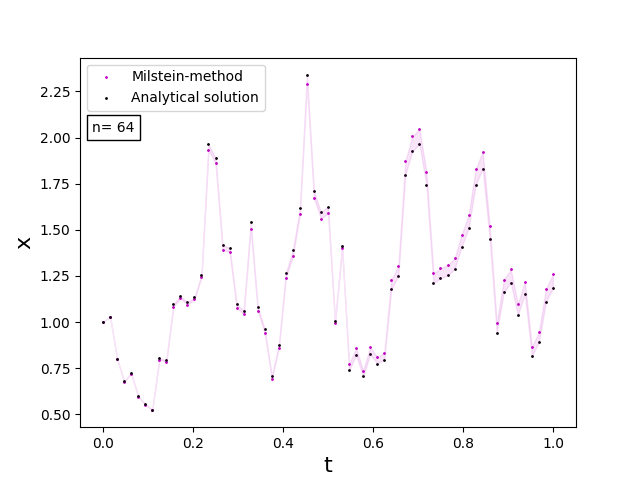
\includegraphics[scale=0.4]{Content/Graphics/Appendix/5gbm3}
   \end{subfigure}
   \begin{subfigure}{0.49\linewidth} \centering
     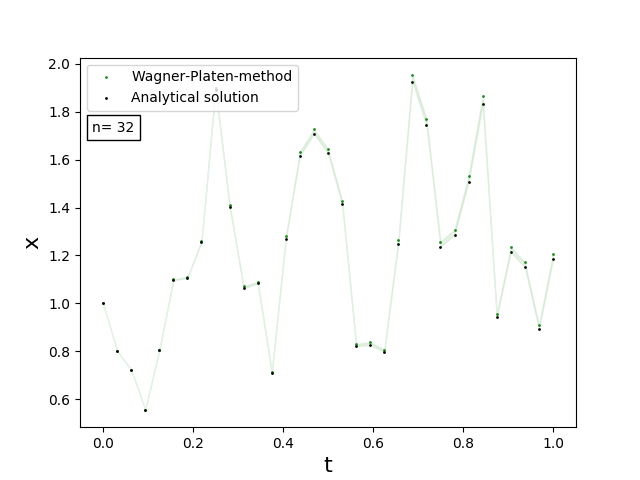
\includegraphics[scale=0.4]{Content/Graphics/Appendix/3gbm3}
   \end{subfigure}
   \begin{subfigure}{0.49\linewidth} \centering
     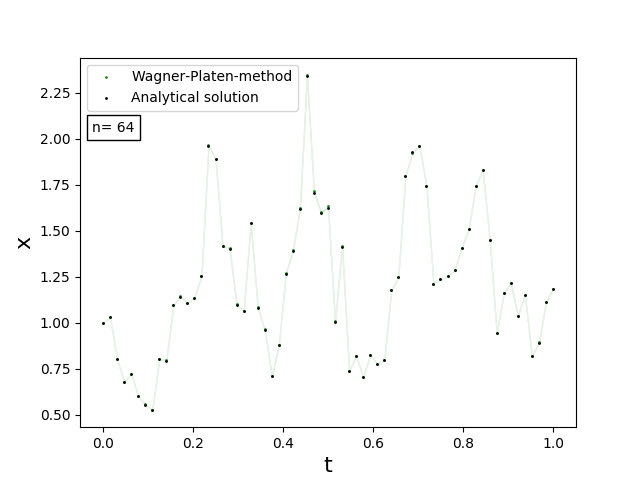
\includegraphics[scale=0.4]{Content/Graphics/Appendix/6gbm3}
   \end{subfigure}
\caption{Approximation (colored dots) of the sample path of the Ornstein-Uhlenbeck process and the true sample path (black dots) for n = 32, 64 using Euler, Milstein and Wagner-Platen.}
\end{figure}


\begin{figure}[!h]
     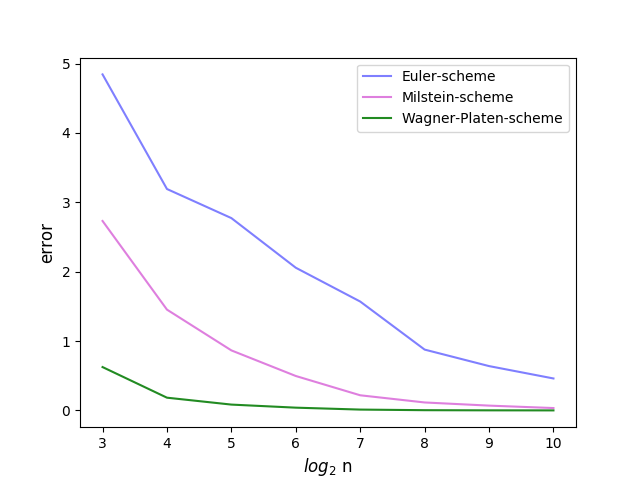
\includegraphics[scale=0.7]{Content/Graphics/Appendix/Error_analysis_gbm}
	\caption{Monte-Carlo estimates of the approximation error and the step amount n (logarithmized) for the geometric Brownian motion using Euler, Milstein, Wagner-Platen (20'000 simulations).}
\end{figure}
\begin{figure}[!h]
     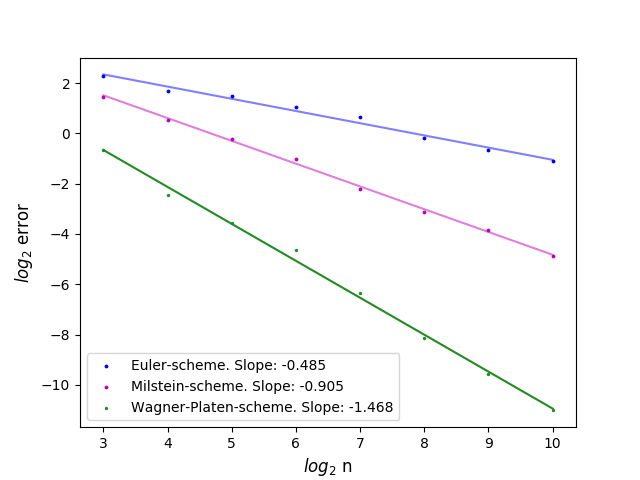
\includegraphics[scale=0.7]{Content/Graphics/Appendix/Conv_order_gbm}
\caption{Log-log plot of the approximation error and the step amount n for the geometric Brownian motion using Euler, Milstein, Wagner-Platen (20'000 simulations).} 
\end{figure}
